% SCRIPT
% The next project in my presentation is named "Physician software interface for an intelligent glucose monitor."

%\renewcommand{\Titulo}{Physician software interface for an intelligent glucose monitor~}

\begin{frame}{\citetitle{MarcoNuno_CongArbIng_2012_01_00}\footnotemark (1)}

% Slide 1
\note[item]{\scriptsize Los pacientes con diabetes tipo 1 o 2 requieren checar varias veces al día sus niveles de glucosa } 
\note[item]{\scriptsize Se requiere de un dispositivo que recomiende dosis de insulina bsado en los parametros fisiológicos del paciente y de los carbohidratos consumidos }
\note[item]{\scriptsize Se desarrolló una plataforma We developed a medical surveillance platform with two components}
\note[item]{\scriptsize The first component is an Intelligent Glucose Monitor (IGM)
with the hardware layer and electronics needed to interact with glucose-sensing strips}
\note[item]{\scriptsize The second one is a Physician software interface (PSI) to configure and extract information from an Intelligent Glucose Monitor (IGM). }

	\begin{itemize}
\item Los pacientes con diabetes tipo 1 o 2 requieren checar varias veces al día sus niveles de glucosa 
\item La mayoría de los dispositivos comerciales almacenan el historia de lecturas de glucosa en el dispositivo.
\item Se desarrollo un monitor de glucosa inteligente (IGM).
\item El médico puede obtener los datos del dispositivo a través de una aplicación de esritorio (PSI).
\item Herramientas:
	\begin{itemize}
		\item C++ para el IGM.
		\item Java para el PSI.
	\end{itemize}
	\end{itemize}
\footnotetext[1]{\fullcite{MarcoNuno_CongArbIng_2012_01_00}}
\setcounter{footnote}{0}
\end{frame}

\begin{frame}{\citetitle{MarcoNuno_CongArbIng_2012_01_00} (2)}


\begin{columns}
		\begin{column}{0.48\textwidth}
		    Componentes
		    \begin{itemize}
		        \item Microcontrolador.
                \item LCD Display.
                \item Sensor de Glucosa.
                \item Real time clock.
                \item Interfaz USB .
                \item Interfaz para obtenr datos de las tiras de sensado de glucosa.
            \end{itemize}
            Un menú permite al usuuario interactuar con el IGM. 
		\end{column}
		
				\begin{column}{0.48\textwidth}
\begin{center}
     \begin{tabular}{c}
         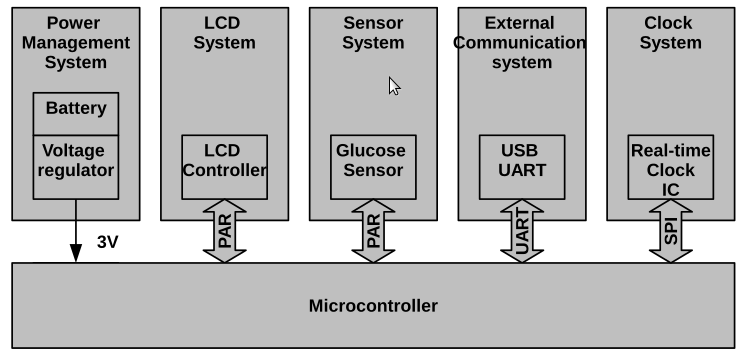
\includegraphics[width=0.85\linewidth]{Figs/IntelligentGlucometer1}\\
         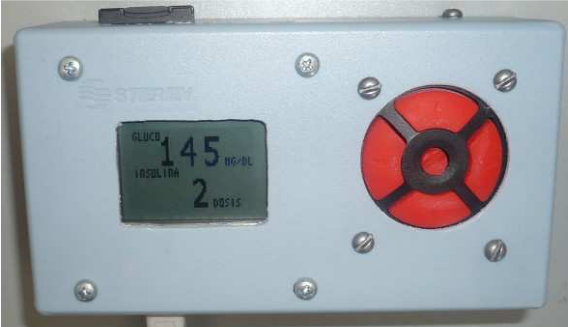
\includegraphics[width=0.75\linewidth]{Figs/IntelligentGlucometer3}\\
          \end{tabular}
\end{center}
		\end{column}
				\end{columns}

\end{frame}



\begin{frame}{\citetitle{MarcoNuno_CongArbIng_2012_01_00} (3)}
\begin{columns}
		\begin{column}{0.48\textwidth}
		La interfaz de médico permite las siguientes acciones:
		\begin{itemize}
		\item Obtener y almacenar los datos de las lecturas de glucosa del IGM, y generar informes.
		\item Configurar el perfil médico del paciente, en base a esto, el IGM recomienda las dosis de insulina		
        \end{itemize}
				\end{column}
				\begin{column}{0.48\textwidth}
\begin{center}
     \begin{tabular}{c}
         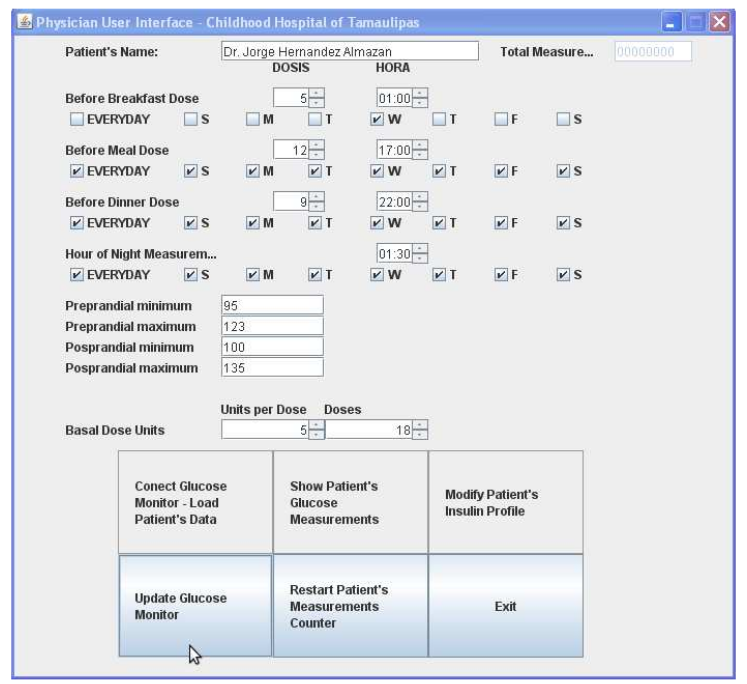
\includegraphics[width=0.86\textwidth]{Figs/IntelligentGlucometer4}
          \end{tabular}
\end{center}
		\end{column}
				\end{columns}
\end{frame}


